\chapter{电路文档}\label{sec8}

在前面章节中介绍电路的目的是帮助读者理解电路原理,所以有些电路仅给出了最简单的例子。在本章中,会直接给出一些电路的结果供参考。对于较难的电路会给出思路。

\section{传感器}
\begin{figure}[!ht]
    \centering
    
\includegraphics{images/221.png}
    \caption{区域重生感应器。在玩家进入世界或玩家复活后,首次进入傀儡附近时激活,有小延迟。}
\end{figure}
\begin{figure}[!ht]
    \centering
    
\includegraphics[width=0.45\textwidth]{images/11.png}
    \qquad
    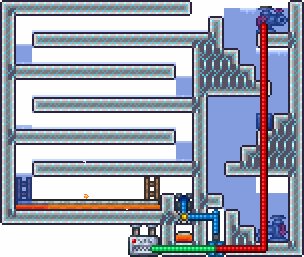
\includegraphics[width=0.45\textwidth]{images/12.png}
    \caption{开服感应器。在玩家进入世界时激活。}
\end{figure}
\begin{figure}[!ht]
    \centering
    
\includegraphics{images/309.png}
    \qquad
    
\includegraphics{images/310.png}
    \caption{血月感应器。打开一秒计时器后,压力板会不断激活。}
\end{figure}
\begin{figure}[!ht]
    \centering
    
\includegraphics{images/311.png}
    \caption{血月\&雨天感应器。打开一秒计时器后,血月时右边火把不断激活,雨天且不是血月时左边火把不断激活。}
\end{figure}
\begin{figure}[!ht]
    \centering
    
\includegraphics{images/312.png}
    \caption{击退感应器。玩家被击退时传送走。用于检测穿墙怪。}
\end{figure}

\section{递次电路}

\section{降频电路}
\subsection{固定数值的降频}
\begin{figure}[!ht]
    \centering
    
\includegraphics{images/327.png}
    \qquad
    
\includegraphics{images/328.png}
    \caption{降频2}
\end{figure}
\begin{figure}[!ht]
    \centering
    
\includegraphics{images/331.png}
    \qquad
    
\includegraphics{images/332.png}
    \caption{降频3}
\end{figure}
\begin{figure}[!ht]
    \centering
    
\includegraphics{images/334.png}
    \qquad
    
\includegraphics{images/333.png}
    \caption{降频4}
\end{figure}
\subsection{交错数值的降频}
\begin{figure}[!ht]
    \centering
    
\includegraphics{images/330.png}
    \qquad
    
\includegraphics{images/329.png}
    \caption{降频1-2}
\end{figure}
\subsection{可变数值的降频}

\section{数字显示}
\begin{figure}[!ht]
    \centering
    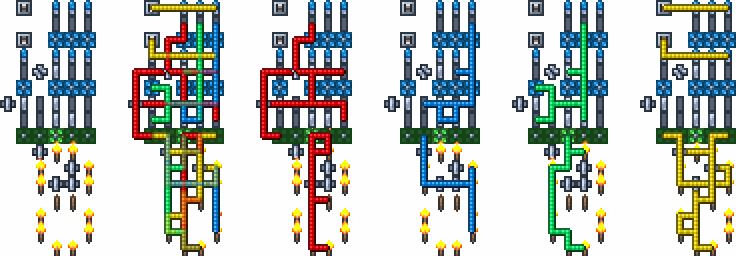
\includegraphics[width=\textwidth]{images/347.png}
    \caption{带复位六进制计数器}
\end{figure}

\section{操纵板}

\begin{figure}[!ht]
    \centering
    
\includegraphics{images/253.png}
    \qquad
    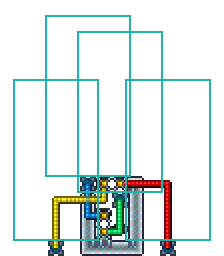
\includegraphics{images/254.png}
    \caption{低频四向操纵板(设计1)}
\end{figure}